\section{Related Work}
\label{sec:related_work}

In this section, we review areas mostly related to our work, \ie, image retrieval and visual place recognition.

\subsection{Image Retrieval}

Image retrieval is a fundamental and well-established task in computer vision that involves searching for images similar to a given query within a large database.
The process of image retrieval typically consists of two stages: global retrieval and re-ranking. In the first stage, a global descriptor that aggregates local features is used to retrieve $k$ candidates from a large database. This is followed by spatial verification through local feature matching to re-rank these $k$ candidates. Early research relied on handcrafted features \cite{Lowe2004DistinctiveIF, BAY2008346}, while current methods utilize deep networks to learn informative representations \cite{cao2020unifyingdeeplocalglobal, radenović2018finetuningcnnimageretrieval}.

Most image retrieval methods focus on selecting diverse relevant images to help users discover options that align with their interests or needs in real-world applications \cite{Wan2014DeepLF}. Although these methods are effective in retrieving similar images, they often lack the emphasis on distinguishing between categories or achieving precise ReID \cite{10.1145/1348246.1348248}.
In \mbox{contrast}, our approach prioritizes achieving accurate ReID. Following a ``global retrieval and re-ranking" pipeline, we first use global context features to identify the top five room candidates. Our object-aware mechanism then refines the search in a coarse-to-fine manner, progressively distinguishing among candidates until the most similar room is \mbox{identified}, yielding accurate results.

\begin{figure*}[ht]
    \centering
    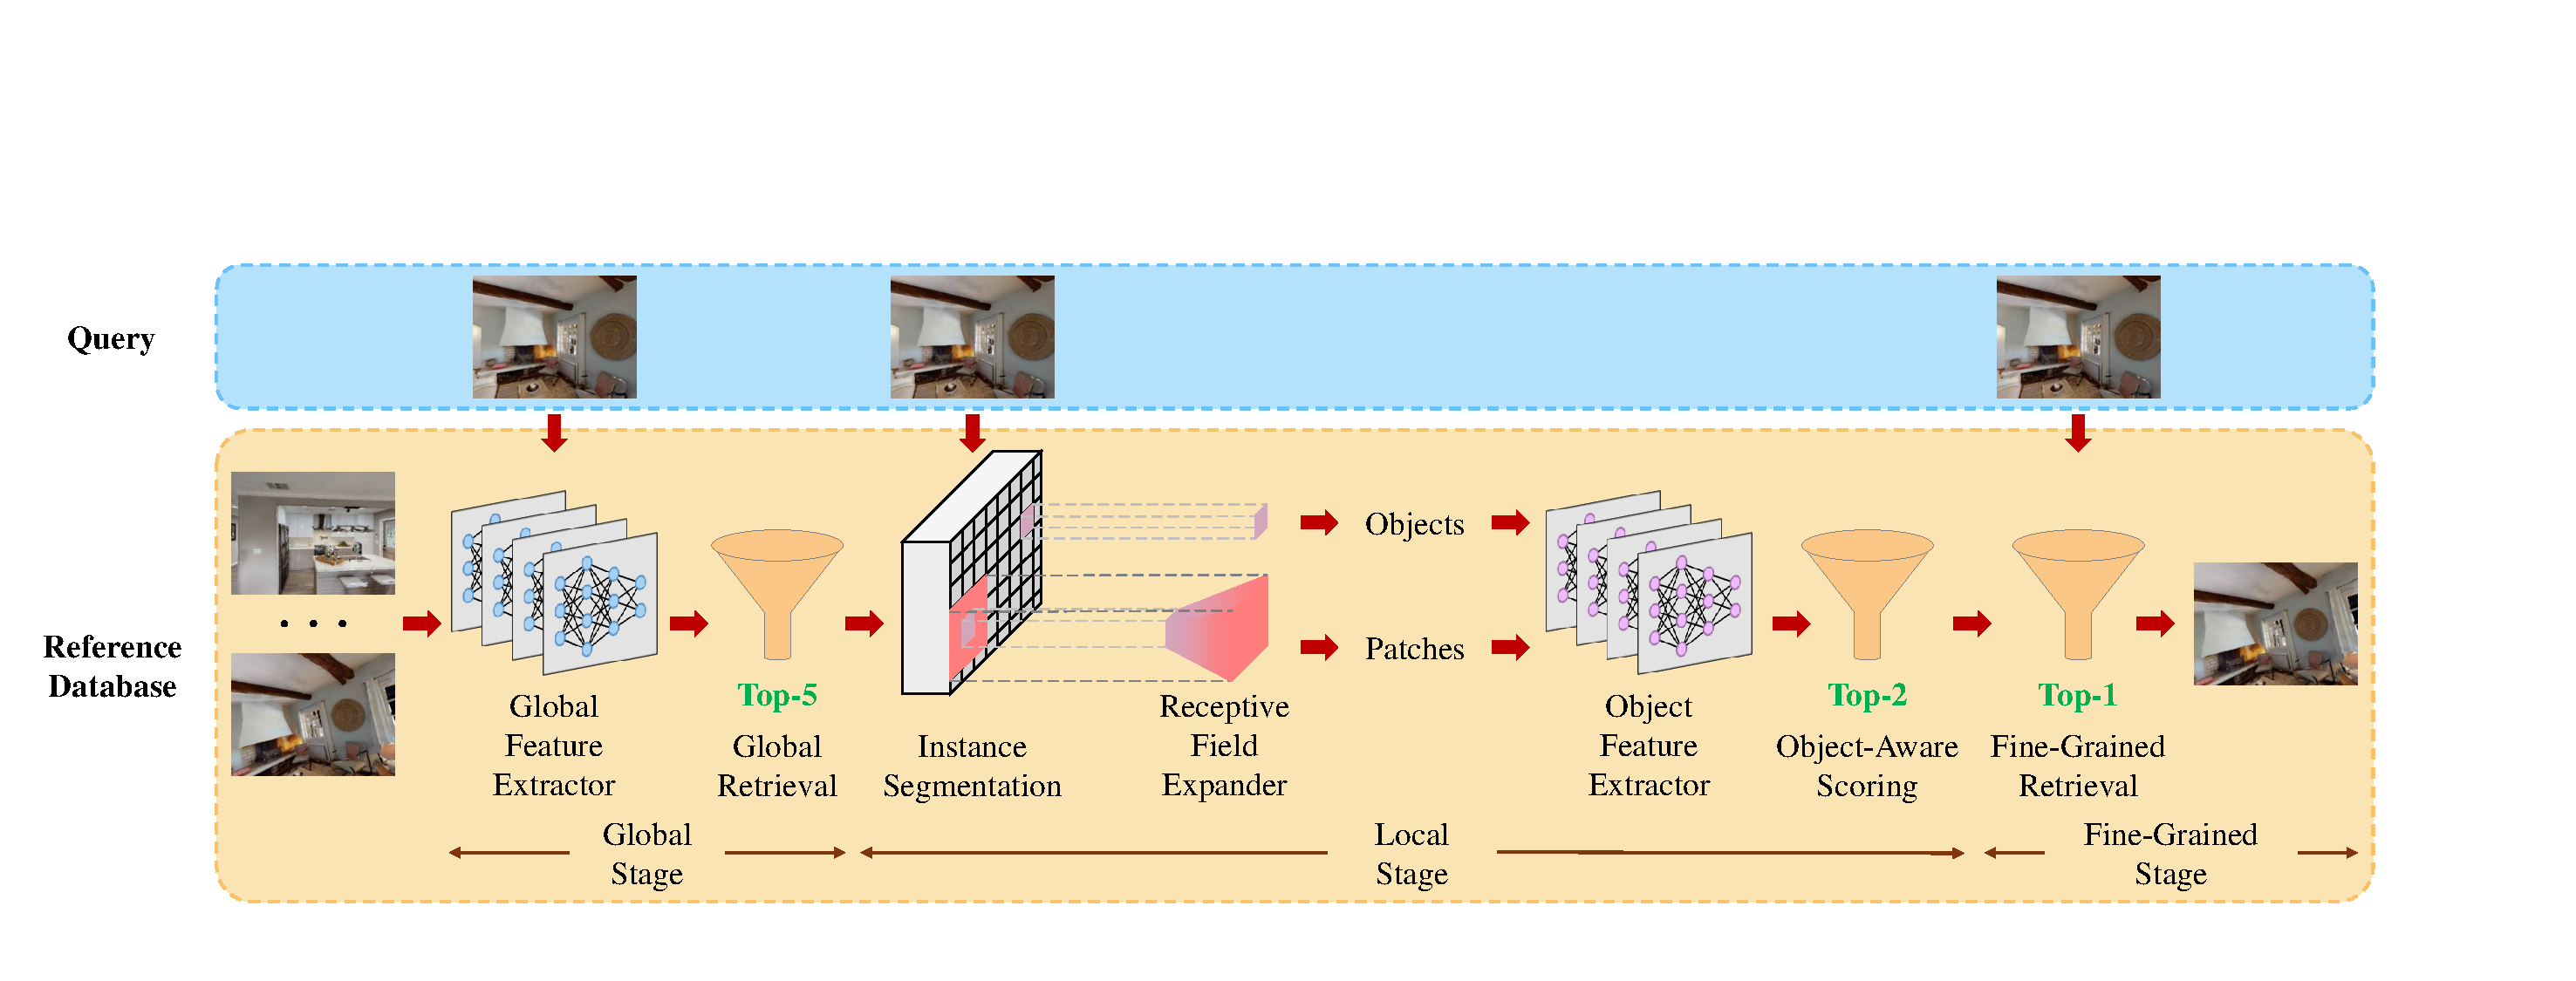
\includegraphics[width=\textwidth]{pipeline_font.pdf}
    \vspace{-16pt}
    \caption{\textbf{The AirRoom coarse-to-fine pipeline}. The pipeline begins with the Global Feature Extractor, which captures global context features to retrieve the top-5 reference images. Instance segmentation then generates object masks, followed by the Receptive Field Expander, which extracts object patches. The Object Feature Extractor processes both object and patch features. The Object-Aware Scoring module narrows the selection to the top-2 candidates, and Fine-Grained Retrieval identifies the most suitable reference image.}
    \vspace{-15pt}
    \label{fig:pipeline}
\end{figure*}

\subsection{Visual Place Recognition}

Visual place recognition (VPR) is often framed as a special image retrieval problem, aiming to match a view of a location with an image of the same place taken under different conditions.
Previous methods fall into two categories: those that directly use global descriptors and those that aggregate local features into a global descriptor. Earlier approaches that relied on global descriptors primarily used CNN-based backbones, such as ResNet \cite{he2015deepresiduallearningimage}, to generate these descriptors. More recent methods, however, leverage foundation models like DINOv2 \cite{oquab2024dinov2learningrobustvisual} for enhanced feature representation. In the aggregation category, early techniques employed handcrafted features like SIFT \cite{Lowe2004DistinctiveIF}, SURF \cite{10.1007/11744023_32}, and ORB \cite{6126544}. Later advancements, including the NetVLAD series \cite{arandjelović2016netvladcnnarchitectureweakly, hausler2021patchnetvladmultiscalefusionlocallyglobal} and AnyLoc \cite{keetha2023anylocuniversalvisualplace}, adopted learning-based models to extract feature maps and combine local features into comprehensive global descriptors.

However, the high performance of most VPR approaches is largely attributed to large-scale training on VPR-specific datasets \cite{keetha2023anylocuniversalvisualplace}. Collecting extensive data for outdoor scenes is relatively straightforward due to natural variations in daylight, weather, and seasons. However, such data collection is more challenging in indoor rooms, making large-scale training on indoor datasets difficult and potentially limiting their effectiveness.
Our approach effectively tackles this challenge by focusing on object-oriented feature representations, allowing us to leverage mature, pre-trained models for object feature learning. This design enables AirRoom to deliver robust performance without requiring any additional training or fine-tuning on specific datasets.
% Our approach addresses this challenge by centering on objects within indoor spaces, leveraging object-related feature representations. Additionally, AirRoom benefits from mature, pre-trained models for object-centric feature learning. This design enables our approach to deliver robust performance without the need for additional training or fine-tuning on specific datasets.